\documentclass{scrreprt}

\usepackage{aligned-overset}
\usepackage{amsmath}
\usepackage{amssymb}
\usepackage{bm}
\usepackage{chngcntr}
\usepackage[shortlabels]{enumitem}
\usepackage{hyperref}
\usepackage[utf8]{inputenc}
\usepackage{mathtools}
\usepackage{physics}
\usepackage{tabularx}
\usepackage{titling}
\usepackage{fancyhdr}
\usepackage{xfrac}
\usepackage[table]{xcolor}
\usepackage{pgfplots}

%% Fix equation numbering for scrreprt class.
\counterwithout{equation}{chapter}

\pgfplotsset{compat = newest}
\usepgfplotslibrary{patchplots}
\usetikzlibrary{intersections}
\usetikzlibrary{shapes}
\usetikzlibrary{shapes.geometric}
\usetikzlibrary{patterns}
\usepgfplotslibrary{fillbetween}

\author{Karsten Lehmann}
\date{SoSe 2021}
\title{Übung 12 Analysis - Weiterführende Konzepte}

\pagestyle{fancy}
\fancyhf{}
\lhead{\thetitle}
\rhead{\theauthor}
\lfoot{\thedate}
\rfoot{Seite \thepage}

\newcommand\skalprod[1]{\left\langle #1 \right\rangle}
\newcommand\nnorm[1]{\left\lvert\left\lvert\left\lvert #1 \right\rvert\right\rvert\right\rvert}

\begin{document}
\setcounter{chapter}{1}
\section*{Extremalaufgaben mit Gleichungsnebenbedingungen}

\paragraph{Aufgabe 1} Ermitteln Sie mit Hilfe der Methode der
Lagrange-Multiplikation diejenigen Punkte $Q = (x, y)$ auf der Hyperbel
$M = \qty{(x, y) \in \mathbb{R}^2 \colon y^2 - x^2 = 1}$, die vom Punkt
$P = (1, 0)$ den kürzesten Abstand haben.
Berechnen Sie den Abstand $d(P, Q)$ von $P$ und $Q$.
Überlegen Sie sich, warum für der ermittelten Punkte tatsächlich der
kürzeste Abstand ermittelt wurde.

\subparagraph{Lösung:} $M = \qty{(x, y) \in \mathbb{R}^2 \colon y^2 - x^2 = 1}$
ist nicht offen.
\begin{center}
  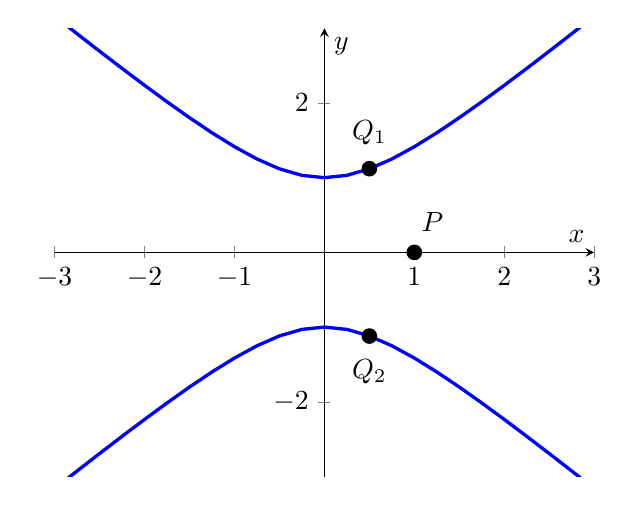
\begin{tikzpicture}
    \begin{axis}[
        axis lines=middle,
        xlabel=$x$,
        xmax = 3,
        xmin = -3,
        ylabel=$y$,
        ymax = 3,
        ymin = -3,
      ]
      \addplot[
        domain = -3:3,
        very thick,
        blue,
      ] {sqrt(x^2 + 1)};
      \addplot[
        domain = -3:3,
        very thick,
        blue,
      ] {-1 * sqrt(x^2 + 1)};
      \node[circle, fill, inner sep=2pt] at (0.5,1.12){};
      \node[circle, fill, inner sep=2pt] at (1,0){};
      \node[circle, fill, inner sep=2pt] at (0.5,-1.12){};
      \node at (1.2, 0.4) {$P$};
      \node at (0.5, 1.6) {$Q_1$};
      \node at (0.5, -1.6) {$Q_2$};
    \end{axis}
  \end{tikzpicture}
\end{center}
$h(x, y) = y^2 - x^2 - 1$ ist stetig differenzierbar.
$M = h^{-1} ({0})$. Aus \textbf{Proposition 6.3.3}
\textit{``Stetige Urbilder abgeschlossener Mengen sind abgeschlossen''} folgt
$M$ ist abgeschlossen.

\textbf{Existieren Extremalstellen von stetigen Funktionen auf $M$?}
\[
  d(\underset{(x, y)}{\underbrace{Q}}, \underset{(1, 0)}{\underbrace{P}})
  = \norm{\overrightarrow{PQ}}_2
  = \qty\Big(\qty(x - 1)^2 + y^2)^{\frac{1}{2}}
\]
\[
  f(x, y) = d(Q, P)^2 = (x - 1)^2 + y^2
\]
$d(\cdot, P)$ und $f$ haben gleiches Monotonieverhalten für $d(\cdot, P) \geq 0$.

\textbf{Problem:} $f(x, y) \longrightarrow \min$ bei $(x, y) \in M$.

Lagrange-Funktion: $F(x, y, \lambda) = f(x, y) + \lambda \cdot h(x, y)$
\begin{itemize}
\item $f, h$ sind stetig differenzierbar mit $\nabla f(x, y) = \begin{pmatrix}
    2 \qty\big(x - 1) \\
    2 y
  \end{pmatrix}$ und $\nabla h(x, y) = \begin{pmatrix}
    -2 x \\
    2 y
  \end{pmatrix}$
\item Regularitäts- / Rangbedingung: Jacobi-Matrix der Nebenbedingung besitzt Vollrang.
  \[
    J_h(x, y) = \nabla h(x, y)^T \ne \begin{pmatrix}0 & 0\end{pmatrix}
  \]
  Es gilt $\nabla h(x, y) = \begin{pmatrix}-2x \\ 2y \end{pmatrix} =
  \begin{pmatrix}0 \\ 0\end{pmatrix} \iff x = y = 0$, aber $(0, 0) \notin M$

  $\Rightarrow$ Rangbedingung gilt.
\end{itemize}

Falls $\qty(\overline{x}, \overline{y})$ eine lokale Extremalstelle von $f$ auf
$M$ ist, so existiert ein $\overline{\lambda} \in \mathbb{R}$, so dass
$\qty(\overline{x}, \overline{y}, \overline{\lambda}) \in M \times \mathbb{R}$
eine freie lokale Extremalstelle von $F$ ist.

$F \colon \mathbb{R}^3 \to \mathbb{R}$ ist stetig differenzierbar.
Notwendige Qptimalitätsbedingung:
$\nabla F(\overline{x}, \overline{y}, \overline{\lambda}) = (0, 0, 0)$.
\setcounter{section}{1}
\begin{align}
  \frac{\partial F}{\partial x} (\ldots) &= 2(x - 1) - 2 \lambda x
  = 2(x(1 - \lambda) - 1) = 0 & \label{eq:1-1} \\
  \frac{\partial F}{\partial y} (\ldots) &= 2y + 2\lambda y = 2y(1 + \lambda) = 0 \label{eq:1-2} \\
  \frac{\partial F}{\partial \lambda} (\ldots) &= h(x, y) = y^2 - x^2 - 1 = 0 \label{eq:1-3}
\end{align}
$\Rightarrow$ nichtlineares Gleichungssystem.

$\hyperref[eq:1-2]{(2)} \iff y = 0 \lor \lambda = -1$

$y = 0$ in $\hyperref[eq:1-3]{(3)}$ einsetzen führt zu $-x^2 - 1 = 0$, nicht lösbar.
$\Rightarrow y \ne 0 \land \lambda = -1$

$\lambda = -1$ in $(1)$ einsetzen: $2x - 1 = 0 \Rightarrow x_1 = \frac{1}{2}$

$x_1 = \frac{1}{2}$ in $\hyperref[eq:1-3]{(3)}$ einsetzen:
$y^2 = \frac{5}{4}, y_{1|2} = \pm \frac{\sqrt{5}}{2}$.

Kritische Punkte: $\qty(x_1, y_1) = \qty(\frac{1}{2}, \frac{\sqrt{5}}{2})$,
$\qty(x_2, y_2) = \qty(\frac{1}{2}, - \frac{\sqrt{5}}{2})$ mit
$f\qty(x_k, y_k) = \frac{3}{2}$ und $d\qty(Q_k, P) = \sqrt{\frac{3}{2}}$.

Wir betrachten
$M_0 \coloneqq M \cap \qty{(x,y) \in \mathbb{R}^2 {\Big |}
  f(x, y) \leq f\qty(x_k, y_k) = \frac{3}{2}}
= h^{-1}(\qty{0}) \cap f^{-1}\left( \left(-\infty, \frac{3}{2}\right] \right)$

$\Rightarrow M_0$ ist abgeschlossen, da $h, f$ stetig und
${0}, {-\infty, \frac{3}{2}}$ abgeschlossen sind.

Angenommen $M_0$ ist nicht beschränkt, dann existiert eine Folge
$\qty(x_n, y_n)_{n \in \mathbb{N}}$ in $M_0$ mit
$\norm{\qty(x_n, y_n)}_2 \overset{n \to \infty}{\longrightarrow} +\infty$,
Widerspruch zu
$\qty(x_n, y_n) \in f^{-1}\left(\left(-\infty, \frac{3}{2}\right]\right)$.

$\Rightarrow M_0$ ist beschränkt und somit kompakt. Nach Weierstraß besitzt
$f$ auf $M_0$ globale Minimalstellen, die auch globale Minimalstellen von
$f$ auf $M$ sind.

$\Rightarrow f$ besitzt lokale Minimalstellen auf $M$

$\Rightarrow$ Diese befinden sich unter den kritischen Punkten.

Wegen $f\qty(x_k, y_x) = \frac{3}{2}$ sind $\qty(x_1, y_1), \qty(x_2, y_2)$
die globalen Minimalstellen.

\newpage
\paragraph{Aufgabe 2} (Ungleichung zwischen geometrischem und arithmetrischem
Mittel).
Beweisen Sie für $z = \qty(z_1, \ldots, z_N) \in \mathbb{R}_{\geq 0}^N$ die
Ungleichung
\[
  A\qty(z_1, \ldots, z_N) \coloneqq \frac{1}{N} \sum_{k = 1}^N z_k \geq
  G\qty(z_1, \ldots, z_N) \coloneqq \sqrt[N]{\prod_{k = 1}^N z_k}
\]
mittels der Methode der Lagrange-Multiplikatoren.
Betrachten Sie dazu folgendes Optimalitätsproblem
\[
  f(x) = f\qty(x_1, \ldots, x_N) \coloneqq \sum_{k = 1}^N x_k \longrightarrow \min
\]
\[
  \text{bei } x \in U \coloneqq \qty{x = \qty(x_1, \ldots, x_N) \in \mathbb{R}^R_{> 0}
    \middle | h(x) \coloneqq \prod_{k = 1}^N x_k - 1 = 0
  }
\]

\subparagraph{Lösung:} $N = 2 \colon \frac{x_1 + x_2}{2} \geq \sqrt{x_1x_2}
\iff x_1^2 + 2 x_1x_2 + x_2^2 \geq 4x_1x_2
\iff x_1^2 - 2x_1x_2 + x_2^2 = (x_1 - x_2)^2 \geq 0, x_{1|2} \geq 0$.

\begin{enumerate}[label={Fall \arabic*:}]
\item $\exists k_0 \colon z_{k_0} = 0 \Rightarrow A\qty(z_1, \ldots, z_N)
  \geq \frac{z_{k_0}}{N} = 0 = G\qty(z_1, \ldots, z_N)$
\item Für alle $z_k$ gilt $z_k > 0 \Rightarrow G\qty(z_1, \ldots, z_N) > 0$
  \[
    z \mapsto x \coloneqq \frac{z}{G(z)} \Rightarrow \prod_{k = 1}^N x_k
    = \prod_{k = 1}^N \frac{z_k}{\qty(\prod_{j = 1}^N z_j)^{\frac{1}{N}}}
    = 1
  \]
  $f(x) = NA(x) \longrightarrow \min$ bei
  $h(x) = \prod_{k = 1}^N x_k - 1 = 0$.
  \begin{itemize}
  \item $f, h$ sind stetig differenzierbar mit
    \[
      \frac{\partial f}{\partial x_k}(x) = 1,
      \frac{\partial h}{\partial x_k}(x) = \frac{1}{x_k} \underset{= 1}{\underbrace{\prod_{j = 1}^N x_j}} = \frac{1}{x_k}
    \]
  \item Rangbedingung:
    \[
      \nabla h(x) = \qty(\frac{1}{x_1}, \ldots, \frac{1}{x_N})
      \ne \qty(0, \ldots, 0)
    \]
    $\Rightarrow$ Rangbedingung erfüllt.
  \newpage
  \item Lagrangefunktion: $F(x, \lambda) = f(x) + \lambda h(x)$
    \setcounter{equation}{0}
    \begin{flalign}
      \frac{\partial F}{\partial x_k}(x) &= 1 + \frac{\lambda}{x_k} = 0
      \quad \text{für } k = 1, \ldots, N \label{eq:2-1} & \\
      \frac{\partial F}{\partial \lambda}(x) &= h(x) = \prod_{k = 1}^N x_k - 1 = 0 \label{eq:2-2}
    \end{flalign}
    $\hyperref[eq:2-1]{(1)} \Rightarrow x_k = - \lambda$ für $k = 1, \ldots, N$
    \[
      \overset{\hyperref[eq:2-2]{(2)}}\Rightarrow h(x) =
      \prod_{k = 1}^N (-\lambda) - 1 = (-\lambda)^N - 1 = 0
    \]
    $\Rightarrow \lambda = -1 \Rightarrow x_k = 1$ für $k = 1, \ldots, N$
  \end{itemize}
  Kritischer Punkt: $\overline{x} = e = (1, \ldots, 1)$.
  Für $\epsilon > 1$ gilt
  $x_{\epsilon} = \qty(\epsilon, \frac{1}{\epsilon}, 1, \ldots, 1) \in M$
  und $f\qty(x_{\epsilon}) \geq \epsilon
  \overset{\epsilon \to \infty}\longrightarrow \infty$.

  $\Rightarrow \overline{x}$ ist kein Maximalpunkt.
  Weitere Untersuchungen zeigen, dass $\overline{x}$ der globale
  Minimalpunkt ist.

  \[
    \Rightarrow f(x) = N \cdot A(x) = N \cdot A\qty(\frac{z}{G(z)})
    = N \frac{A(z)}{G(z)} \geq f(\overline{x}) = N
  \]
  $\Rightarrow A(z) \geq G(z)$
\end{enumerate}

\paragraph{Aufgabe 3} Sei $f \colon \mathbb{R}^2 \to \mathbb{R}$ definiert durch
$f(x, y) \coloneqq x^2 + xy + y^2$.
Weiter sei $M \coloneqq \qty{(x, y) \in \mathbb{R}^2 {\Big |} x^2 + y^2 \leq 1}$.
Ermitteln Sie $f_{\min} = \min_{(x, y) \in M} f(x, y)$ und
$f_{\max} = \max_{(x, y) \in M} f(x, y)$

\subparagraph{Lösung:} $M = \mathring{M} \cup \partial$.
Mit $h(x, y) = x^2 + y^2 - 1$ gilt $\mathring{M} = h^{-1}\qty\big((-\infty, 0))$, \\
$\partial M = h^{-1}(\qty{0})$ und $M = h^{-1}\big( (-\infty, 0]\big)$.
Weiterhin ist $h$ stetig $\Rightarrow \mathring{M}$ ist offen, $\partial M$ und
$M$ sind abgeschlossen.

$M$ und $\partial M$ sind beschränkt $\Rightarrow$ kompakt.
Weiterhin ist $f$ stetig $\Rightarrow f$ besitzt auf $M$, $\partial M$
globale Extremstellen.
\begin{itemize}
\item lokale Extremstellen auf $\mathring{M}$ ermitteln.

  Notwendige Bedingung: $\nabla f(x, y) = \begin{pmatrix}
    2x + y \\
    x + 2y
  \end{pmatrix} = \underset{A \text{ mit } \det A = 3 \ne 0}{
    \underbrace{\begin{pmatrix}
        2 & 1 \\
        1 & 2
      \end{pmatrix}}
  } \cdot \begin{pmatrix}
    x \\
    y
  \end{pmatrix} = 0$

  $\Rightarrow \begin{pmatrix}
    \overline{x} \\
    \overline{y}
  \end{pmatrix} = A^{-1} \begin{pmatrix} 0 \\ 0\end{pmatrix} =
  \begin{pmatrix} 0 \\ 0\end{pmatrix}$

  Weiter gilt $H_f (x, y) = \begin{pmatrix}
    2 & 1 \\
    1 & 2
  \end{pmatrix}$ mit $\det H_f(x, y) = 3 > 0$.

  $\Rightarrow H_f(x, y)$ ist auf $\mathbb{R}^2$ positiv definit
  ($f$ ist konvex)

  $\Rightarrow (\overline{x}, \overline{y})$ ist lokale Minimalstelle mit
  $f(\overline{x}, \overline{y}) = 0$.

\item lokalle Extremstellen auf $\partial M$ ermitteln.

  Lagrangefunktion: $F(x, y, \lambda) = f(x, y) + \lambda h(x, y)$
  \begin{itemize}
  \item $f, h$ sind stetig differenzierbar
  \item Rangbedingung: $\nabla h(x, y) = \begin{pmatrix}
      2x \\
      2y
    \end{pmatrix} = \begin{pmatrix}
      0 \\
      0
    \end{pmatrix} \iff x = y = 0$, aber $(0, 0) \notin \partial M$

    $\Rightarrow$ Rangbedingung gilt.
  \end{itemize}
  $\Rightarrow$ der Satz von Lagrange ist anwendbar.
  \setcounter{equation}{0}
  \begin{flalign}
    \frac{\partial F(\ldots)}{\partial x} &= 2x (1 + \lambda) + y = 0 \label{eq:3-1} & \\
    \frac{\partial F(\ldots)}{\partial y} &= 2y (1 + \lambda) + x = 0 \label{eq:3-2} \\
    \frac{\partial F(\ldots)}{\partial \lambda} &= x^2 + y^2 - 1 = 0 \label{eq:3-3}
  \end{flalign}
  Angenommen es gilt $x = 0 \overset{\hyperref[eq:3-1]{(1)}}\Rightarrow y = 0
  \overset{\hyperref[eq:3-3]{(3)}}\Rightarrow -1 = 0$, Widerspruch.

  Angenommen es gilt $y = 0 \overset{\hyperref[eq:3-2]{(2)}}\Rightarrow x = 0
  \overset{\hyperref[eq:3-3]{(3)}}\Rightarrow -1 = 0$, Widerspruch.

  $\Rightarrow x \ne 0, y \ne 0$.
  \begin{flalign*}
    \hyperref[eq:3-1]{(1)} \cdot y &= \hyperref[eq:3-2]{(2)} \cdot x & \\
    2xy (1 + \lambda) + y^2 &= 0 = 2xy (1 + \lambda) + x^2 \\
    y^2 &= x^2 \iff \abs{y} = \abs{x} \iff y = \pm x \\
    \hyperref[eq:3-3]{(3)} &\Rightarrow h(x, \pm x) = 2x^2 - 1 = 0 \Rightarrow x_{1|2} = \pm \frac{1}{\sqrt{2}}
  \end{flalign*}
  Kritische Punkte:
  \begin{enumerate}[
    labelindent=*,
    leftmargin=*,
    label={$\qty(x_{\arabic*}, y_{\arabic*}) = $}]
  \item $\frac{1}{\sqrt{2}} (1, 1)$
  \item $-\frac{1}{\sqrt{2}} (1, 1)$
  \item $\frac{1}{\sqrt{2}} (1, -1)$
  \item $\frac{1}{\sqrt{2}} (-1, 1)$
  \end{enumerate}
  mit $f\qty(x_1, y_1) = f\qty(x_2, y_2) = \frac{3}{2}$ und
  $f\qty(x_3, y_3) = f\qty(x_4, y_4) = \frac{1}{2}$.

  Da die globalen Extremalstellen kritische Punkte sein müssen, sind
  $\qty(x_1, y_1), \qty(x_2, y_2)$ die globalen Maximalstellen von
  $f$ auf $\partial M$ und  $\qty(x_3, y_3), \qty(x_4, y_4)$ die globalen
  Minimalstellen von $f$ auf $\partial M$.

\item Vergleich von $f$ auf $\mathring{M}$ und $f$ auf $\partial M$

  $\Rightarrow (\overline{x}, \overline{y}) = (0, 0)$ ist der globale
  Minimalpunkt von $f$ auf $M$, $\qty(x_1, y_1), \qty(x_2, y_2)$ sind
  globale Maximalpunkte von $f$ auf $M$.
\end{itemize}

\section*{Kurvenintegrale und Integrabilitätsbedingungen}
\paragraph{Aufgabe 5:} Gegeben seien $a > b > 0$.
Weiter sei $c = \frac{\sqrt{a^2 - b^2}}{b}$.
Die Kurve $\Gamma$ sei die Schnittkurve des elliptischen Zylinders
$\frac{x^2}{a^2} + \frac{y^2}{b^2} = 1$ mit der Ebene $z - c y = 0$.
Weiterhin sei ein Kraftfeld $f \colon \mathbb{R}^3 \to \mathbb{R}^3$ gegeben
durch $f(x, y, z) \coloneqq (aby, abx, z)$
\subparagraph{Lösung:} $\pi \colon t_0 = a < t_1 < \ldots < t_N = b$
  sei eine Zerlegung von $[a, b]$.
  \[
    \text{Var}_{[a, b]}(\gamma, \pi) = \sum_{k = 1}^N\norm{\gamma(t_k) - \gamma(t_{k - 1})}_2
  \]
  \begin{center}
    \begin{tikzpicture}
      \begin{axis}[
          axis lines=middle,
          xlabel=$x(t)$,
          xmax = 3,
          xmin = -0.4,
          xticklabels={,,}
          ylabel=$y(t)$,
          ymax = 3,
          ymin = -0.4,
          yticklabels={,,}
        ]
        \addplot[
          domain = 0.7:2.7,
          very thick,
          blue,
          samples=30,
        ] {2 - (x - 2)^2};
        \node[circle, fill, inner sep=2pt] at (0.7,0.31){};
        \node[circle, fill, inner sep=2pt] at (1,1){};
        \node[circle, fill, inner sep=2pt] at (2,2){};
        \node[circle, fill, inner sep=2pt] at (2.7,1.51){};
        \node at (1, 0.4) {$\gamma\qty(t_0)$};
        \node at (0.8, 1.2) {$\gamma\qty(t_1)$};
        \node at (2.2, 2.2) {$\gamma\qty(t_1)$};
        \node at (2.5, 1.3) {$\gamma\qty(t_N)$};
      \end{axis}
    \end{tikzpicture}
  \end{center}
  \[
    L(\gamma) = \text{Var}_{[a, b]}(\gamma) = \sup\qty{\text{Var}_{[a, b]}(\gamma, \pi) {\Big |} \pi \in \Pi_{[a, b]}} < \infty
  \]
  $\gamma$ besitzt endliche Variation (rektifizierbar).

  $\gamma \colon [a, b] \to \mathbb{R}^N$ ist stetig differenzierbar.

  $\Rightarrow L(\gamma) = \int_a^b \norm{\gamma'(t)}_2 \,dt$

  Sei $f \colon \mathbb{R}^N \to \mathbb{R}$ stetig und
  $\gamma \colon [a, b] \to \mathbb{R}^N$ stetig differenzierbar.
  \[
    \int_{\gamma} f\,dx = \int_a^b f(\gamma(t)) \cdot \gamma'(t)\,dt
  \]
\begin{enumerate}[a)]
\item Parametrisieren Sie die Schnittkurve mittels elliptischer Polarkoordinaten
  $\gamma(t), t \in [-\pi, \pi]$.
  Zeigen Sie, dass $\gamma'$ und $\gamma''$ senkrecht aufeinander stehen.

  \subparagraph{Lösung:} $Z = \qty{(x,y,z) \in \mathbb{R}^3 {\Big |}
    \frac{x^2}{a^2} + \frac{y^2}{b^2} = 1}$

  $E = \qty{(x,y,z) \in \mathbb{R}^3 {\Big |} Z - cy = 0}$

  $\Gamma = Z \cap E$

  Mit $F(x, y, z) = \begin{pmatrix}
    \frac{x^2}{a^2} + \frac{y^2}{b^2} - 1 \\
    Z - cy
  \end{pmatrix} = \begin{pmatrix}
    0 \\
    0
  \end{pmatrix}$ gilt $\Gamma = \qty{
    (x, y, z) \in \mathbb{R}^3 {\Big |} F(x, y, z) = \begin{pmatrix}
      0 \\
      0
    \end{pmatrix}
  }$

  Elliptische Polarkoordinaten: $x(t) = a \cos t$,
  $y(t) = b \sin t, t \in [-\pi, \pi]$.
  \begin{center}
    \begin{tikzpicture}
      \begin{axis}[
          axis lines=middle,
          xlabel=$x$,
          xmax = 3,
          xmin = -3,
          xticklabels={,,}
          ylabel=$y$,
          ymax = 2,
          ymin = -2,
          yticklabels={,,}
        ]
        \node[
          draw,
          ellipse,
          minimum height = 3cm,
          minimum width = 5cm,
        ] at (0, 0) {};
        \node at (2.5, -0.2) {$a$};
        \node at (-2.5, 0.2) {$-a$};
        \node at (0.4, 1.3) {$b$};
        \node at (0.4, -1.3) {$-b$};
      \end{axis}
    \end{tikzpicture}
  \end{center}
  \[
    Z = \qty{
      (x, y, z) \in \mathbb{R}^3
      {\Big |}
      x(t) = a \cos t,
      y(t) = a \sin t,
      z \in \mathbb{R},
      t \in [-\pi, \pi]
    }
  \]
  $\Rightarrow \gamma(t) = \begin{pmatrix}
    x(t) \\
    y(t) \\
    cy(t)
  \end{pmatrix} = (a \cos t, b \sin t, bc \sin t), t \in [-\pi, \pi]$
  \[
    \norm{\gamma(t)}_2^2 = a^2\cos^2t + b^2\sin^2t +
    (\underset{a^2-b^2}{\underbrace{bc}})^2 \sin^2t = a^2
  \]
  $\Rightarrow \norm{\gamma(t)}_2 = a, t \in [-\pi, \pi]$

  Für $g(t) = \norm{\gamma'(t)}_2^2 = \gamma'(t) \cdot \gamma'(t), t \in [-\pi, \pi]$
  ist differenzierbar mit $g'(t) = \gamma''(t) \cdot \gamma''(t)$.
  Weiter gilt
  \begin{flalign*}
    \gamma'(t) &= \qty\Big(-a \sin t, b \cos t, bc \cos t) & \\
    \Rightarrow  \norm{\gamma'(t)}_2^2 &= a^2 \sin^2 t + b^2 \cos^2 t + bc \cos^2t = a^2 \\
    \Rightarrow g'(t) &= \gamma''(t) \cdot \gamma'(t) = 0
    \Rightarrow \gamma''(t) \perp \gamma'(t)
  \end{flalign*}

\item Ermitteln Sie die Variation dieser Kurve.
  \subparagraph{Lösung:}
  \[
    L(\gamma) = \int_{-\pi}^{\pi} \norm{\gamma'(t)}_2\,dt = 2 \cdot \pi \cdot a
  \]
\end{enumerate}

\end{document}